\documentclass[a4paper,11pt,onecolumn,twoside]{article}

\usepackage{xeCJK}       % 使用XeLaTeX编译
\usepackage{CJK}
\usepackage{fancyhdr}
\usepackage{amsmath,amsfonts,amssymb,graphicx}
\usepackage{graphics}
\usepackage{subfigure}
\usepackage{indentfirst}
\usepackage{bm}          % 公式中的粗体字符(用命令\boldsymbol)
\usepackage{multicol}    % Two cols
\usepackage{abstract}

% For MATLAB Code
\usepackage{listings}
\usepackage[T1]{fontenc}
\usepackage{bigfoot}    % to allow verbatim in footnote
\usepackage[numbered,framed]{matlab-prettifier}



% 下面的命令重定义页面边距

\addtolength{\topmargin}{-54pt}
\setlength{\oddsidemargin}{-0.9cm}  % 3.17cm - 1 inch
\setlength{\evensidemargin}{\oddsidemargin}
\setlength{\textwidth}{17.00cm}
\setlength{\textheight}{24.00cm}    % 24.62
\setCJKmainfont[BoldFont=SimHei,ItalicFont={[stkaiti.ttf]}]{SimSun}

\newfontfamily\kai{STKaiti}          % 楷体
\newfontfamily\hei{SimHei}           % 黑体


\renewcommand{\baselinestretch}{1.1} %定义行间距
\parindent 22pt %重新定义缩进长度



\title{\huge{DSP第二次大作业报告:\\OFDM系统仿真}
\thanks{本文为 \textbf{数字信号处理} 课程第二次大作业报告,提交日期为2017.6.14.}}
\author{杨宇喆 \\[2pt]
\normalsize
1400012996 \qquad yuzhe.yang@pku.edu.cn
\\[2pt]}

\date{}  % 这一行用来去掉默认的日期显示


% ==================================首页页眉页脚定义

\fancypagestyle{plain}{
\fancyhf{}
\lhead{School of EECS\\
\scriptsize{Peking University}}
\chead{\centering{DSP第二次大作业报告\\
\scriptsize{\textbf{Report of Second Project, Digital Signal Processing}}}}
\rhead{1400012996\\
\scriptsize{yuzhe.yang@pku.edu.cn}}
\lfoot{}
\cfoot{}
\rfoot{}}



% ================================R,C,L分别代表左中右,O,E代表奇偶页

\pagestyle{fancy}
\fancyhf{}
\fancyhead[R]{杨宇喆 1400012996}
\fancyhead[C]{DSP第二次大作业报告:OFDM系统仿真}
\fancyhead[L]{\thepage}
\lfoot{}
\cfoot{}
\rfoot{}


\newenvironment{figurehere}
  {\def\@captype{figure}}
  {}
\makeatother



\begin{document}

\newcommand{\supercite}[1]{\textsuperscript{\cite{#1}}}

\maketitle

%  恢复正文页边距
\setlength{\oddsidemargin}{-.5cm}  % 3.17cm - 1 inch
\setlength{\evensidemargin}{\oddsidemargin}
\setlength{\textwidth}{17.00cm}
%\CJKfamily{song}

% one side


\iffalse
% ===================================插入图片格式 //暂时无标题
\begin{center}
    \includegraphics[width=1\textwidth]{test.jpg}
\end{center}

% ===================================插入Matlab代码格式,参考matlab-prettifier文档
\begin{lstlisting}[style=Matlab-editor,
                   basicstyle=\mlttfamily,
                   caption={My 1st Code}, label=code1]
while `\mlplaceholder{condition}`
    if `\mlplaceholder{something-bad-happens}`
        break
    else
    % do something useful
    end
end
\end{lstlisting}
\fi


\section{实验原理概述}

\subsection{$DFT$与$FFT$简介}
离散傅里叶变换~(Discrete Fourier Transform,缩写为$DFT$),是傅里叶变换在时域和频域上都呈离散的形式,将信号的时域采样变换为其$DTFT$的频域采样~\supercite{wiki}。在形式上,变换两端(时域和频域上)的序列是有限长的,而实际上这两组序列都应当被认为是离散周期信号的主值序列。即使对有限长的离散信号作$DFT$,也应当将其看作其周期延拓的变换。在实际应用中通常采用快速傅里叶变换~(Fast Fourier Transform, $FFT$)计算$DFT$。$FFT$是计算序列的离散傅里叶变换~($DFT$)或其逆变换的一种算法~\supercite{wiki}。傅里叶分析将信号从原始域(通常是时间或空间)转换到频域的表示或者逆过来转换。$FFT$会通过把$DFT$矩阵分解为稀疏(大多为零)因子之积来快速计算此类变换~\supercite{wikifft}。

对于$N$点序列 $\left\{x(n)\right\}_{0\leq n<N}$,它的离散傅里叶变换$DFT$为
\begin{equation}
X(k) = \sum_{n=0}^{N-1} x(n) exp(-j\frac{2\pi}{N} nk), \quad k = 0,1,\cdots,N-1.
\end{equation}
离散傅里叶变换的逆变换$IDFT$为:
\begin{equation}
x(n) = \frac{1}{N} \sum_{k=0}^{N-1} X(k) exp(j\frac{2\pi}{N} nk), \quad n = 0,1,\cdots,N-1.
\end{equation}

\subsection{OFDM系统概述}
OFDM,即正交频分复用~(Orthogonal frequency-division multiplexing),有时又称为分离复频调制技术~(discrete multitone modulation, DMT),可以视为多载波传输的一个特例,具备高速率资料传输的能力,加上能有效对抗频率选择性衰减,而逐渐获得重视与采用~\supercite{wiki}。
正交频分复用属于多载波传输技术,所谓多载波传输技术指的是将可用的频谱分割成多个子载波,每个子载波可以载送一低速数据流。OFDM允许各个子载波部分交叠,从而提高频谱利用效率;OFDM信号带宽取决于子载波数量,故具有很好的带宽扩展性~\supercite{ta}。

OFDM的优点有~\supercite{wiki}:
\begin{enumerate}
\item 有效减少多径及频率选择性信道造成接收端误码率上升的影响;
\item 利用适应性调制及编码,可有较佳的传输速度;
\item 接收端可利用简单一阶均衡器补偿通道传输的失真;
\item 频谱效率上升;
\item 有较佳的抵抗``深度衰减''之能力。
\end{enumerate}

\subsubsection{OFDM原理}
OFDM利用数个(2的次方)正交的子载波传送信号。OFDM便是多载波调制的特例,其使用数个正交载波调制信号,在每个子载波间不需要有保护间隔,大大的增加了带宽使用效率,且使OFDM更有位分配的概念,即通道环境好的子载波就加大该载波的power或提高调制等级(e.g., BPSK $\rightarrow$ QAM),位分配使得OFDM带宽使用效率更加高。

经过多载波调制,一个OFDM符号可以表示为
\begin{equation}
s(t) = \sum_{k=0}^{N-1} X(k) \exp({j2\pi f_p t}), \quad f_k = k \triangle f ,\ \triangle f =\frac{1}{T},
\label{form}
\end{equation}
其中$T$为一个OFDM符号的时间长度,$X(k)$表示在第$k$个子载波上所传输的信息。OFDM各个子载波互相交叠,但是各个子载波之间同时满足正交性,即有
\begin{equation}
\int x(t)\ast y(t) dt = \int X(f)Y(f) df = 0.
\end{equation}

\subsubsection{OFDM实现过程}
由公式~\ref{form},不难推出OFDM可以用DFT~(FFT)技术来实现,具体推导如下:
\begin{equation*}
\begin{split}
s(t) & = \sum_{k=0}^{N-1} X(k) \exp({j2\pi f_k t}), \\
s(nT_s) & = \sum_{k=0}^{N-1} X(k)\exp({j2\pi f_k nT_s}),
\end{split}
\end{equation*}
取$f = \frac{1}{NT_s}$,$f_k=kf$,则有
\begin{equation}
x(n) = s(nT_s) = \sum_{k=0}^{N-1} X(k)\exp(\frac{j2\pi k n}{N}).
\end{equation}

OFDM调制可以通过FFT和IFFT算法实现,发送端$N$个信息符号经过IDFT变换构成一个OFDM符号,接收端对一个OFDM符号进行DFT变换构成$N$个待解调的信息符号。综上所述,现给出OFDM系统实现的流程图如下。

\begin{center}
    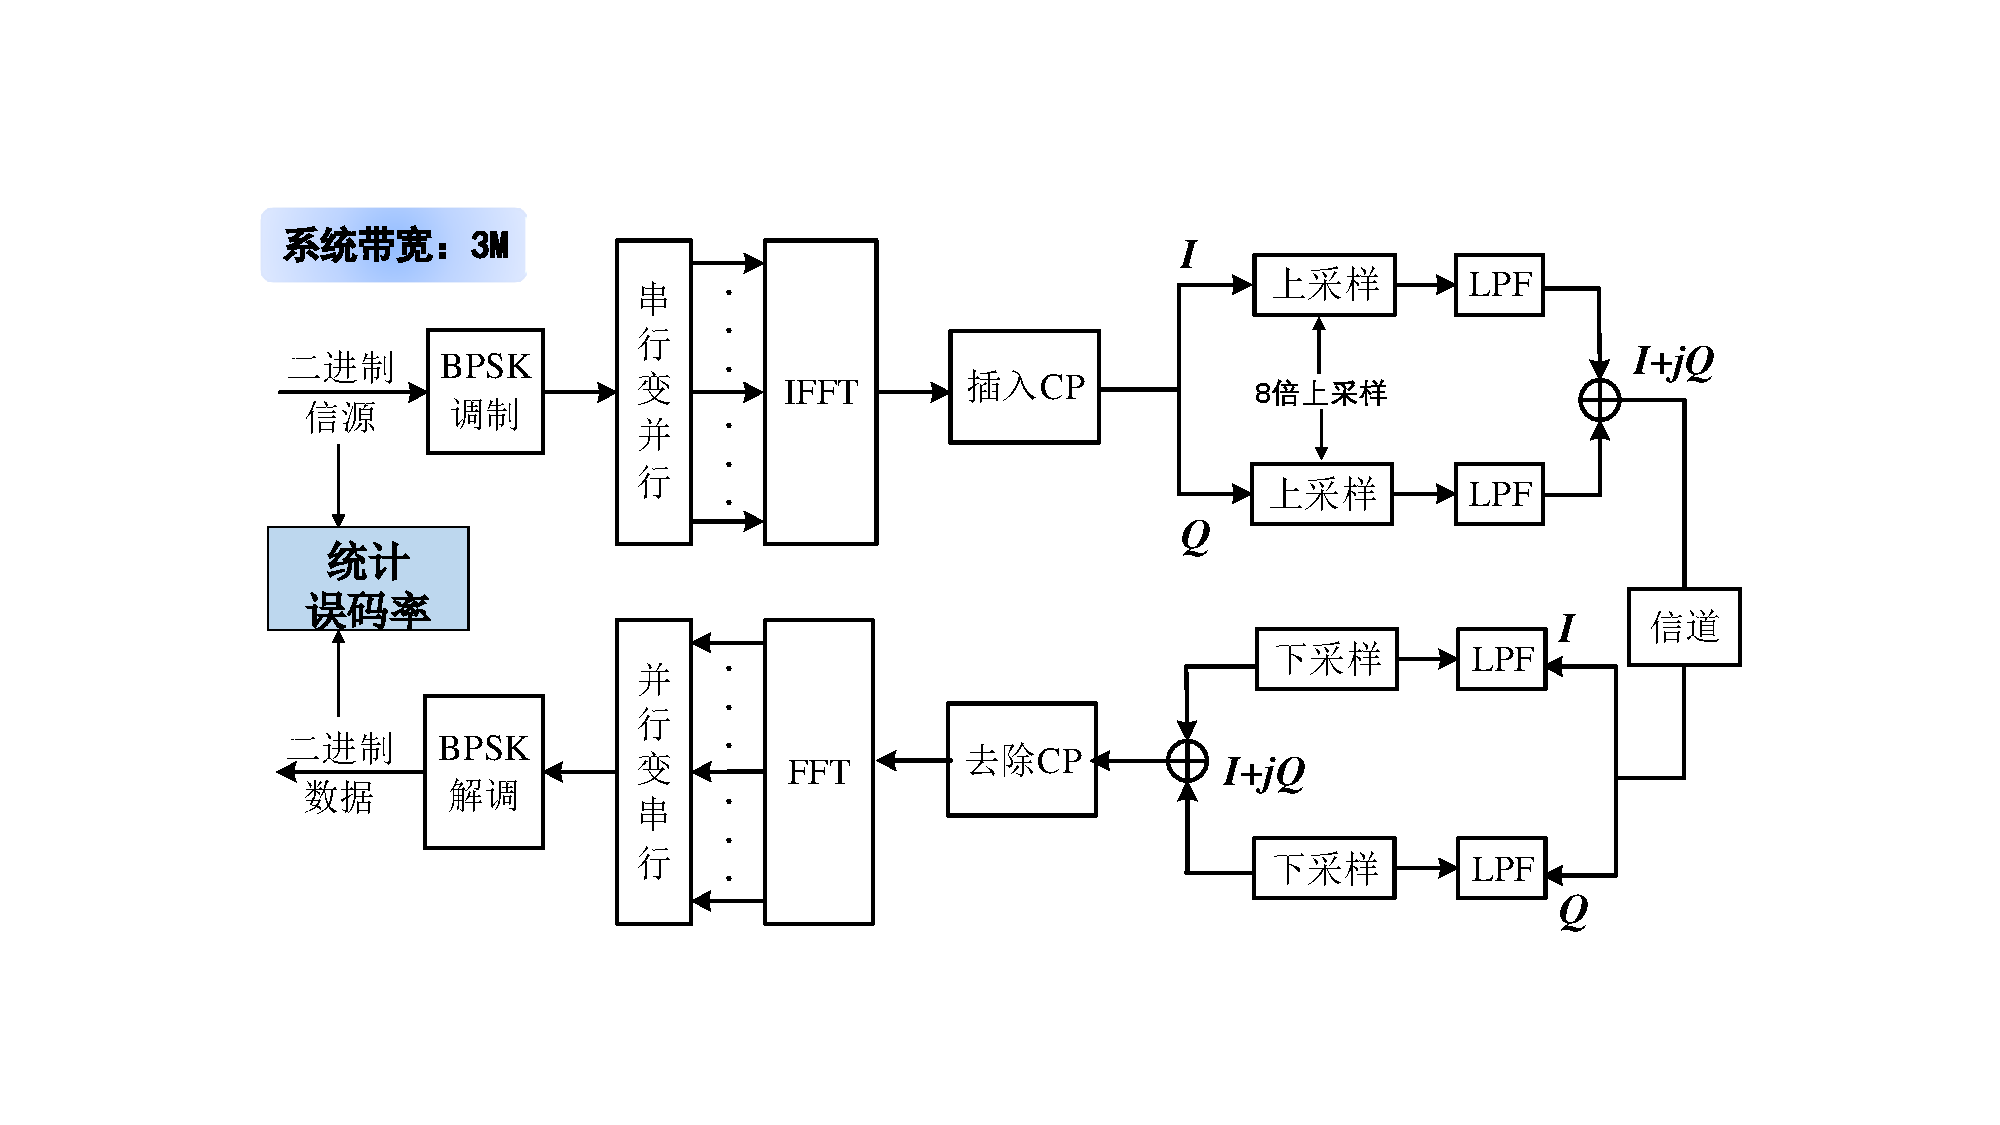
\includegraphics[width=1\textwidth]{system.pdf}
\end{center}

本系统利用BPSK调制,加入了循环前缀~(Cyclic Prefix, CP)来对抗码间串扰~(ISI)和子载波间干扰~(ICI)~\supercite{wiki,ta},后经过上采样,通过设计好的低通FIR滤波器,发射进入加性高斯信道~\supercite{ta}。之后经过一系列逆过程完成信息的解调,从而实现传输过程。

\subsection{FIR数字滤波器概述}
数字滤波器是对数字信号进行滤波处理以得到期望的响应特性的离散时间系统~\supercite{wiki}。作为一种电子滤波器,数字滤波器与完全工作在模拟信号域的模拟滤波器不同。数字滤波器工作在数字信号域,它处理的对象是经由采样器件将模拟信号转换而得到的数字信号。

线性移不变的数字滤波器包括无限长脉冲响应滤波器~(IIR滤波器)和有限长脉冲响应滤波器~(FIR滤波器)两种。这两种滤波器的系统函数可以统一以$Z$变换表示为~\supercite{textbook}:

\begin{equation}
H(z) = \frac{B(z)}{A(z)} = \frac{b_0+b_1 z^{-1}+b_2 z^{-2}+\cdots +b_N z^{-N}}{1+a_1 z^{-1}+a_2 z^{-2}+\cdots +a_M z^{-M}}.
\end{equation}

有限冲激响应~(Finite impulse response, FIR)滤波器是数字滤波器的一种,简称FIR数字滤波器~\supercite{course1}。这类滤波器对于脉冲输入信号的响应最终趋向于0,因此是有限的,而得名~\supercite{wiki,course1}。它是相对于无限冲激响应~(IIR)滤波器而言。由于无限冲激响应滤波器中存在反馈回路,因此对于脉冲输入信号的响应是无限延续的。

有限冲激响应滤波器是一线性系统,输入信号,$x(0),x(1),...,x(n)$,经过该系统后的输出信号,$y(n)$可表示为~\supercite{course2}:
\begin{equation}
y(n) = h_0 x(n) + h_1 x(n-1) + \cdots + h_N x(n-N).
\end{equation}

有限冲激响应滤波器的传递函数可由其冲激响应的$z$变换获得~\supercite{course3}:
\begin{equation}
H(z) = Z\{h(n)\} = \sum_{n=- \infty}^{\infty} h(n) z^{-n} = \sum_{n=0}^{N} h(n) z^{-n}.
\end{equation}


\section{实验过程及数据}

\subsection{系统参数设置}
本次OFDM仿真试验中,仿真参数设置如下表格$Matlab$代码所示:

% ===================================插入Matlab代码格式,参考matlab-prettifier文档
\begin{lstlisting}[style=Matlab-editor,
                   basicstyle=\mlttfamily,
                   caption={Parameter Set up}, label=code1]
nFFT = 128;             % n点fft的长度
nBpsk_Ofdm = 128;       % 每个OFDM符号带有的BPSK符号
nBit_Sym = 128;         % 每个OFDM符号所带的bit数目(对于BPSK而言和 nBpsk_Ofdm 一样)
nSym = 10^4;            % OFDM 符号数目(bit number > 10^5,即symbol > 10^3,此处取10^4保证数目精确度)
EbN0dB = 0:0.5:12;      % Bit to Noise Ratio
EsN0dB = EbN0dB + 10*log10(nBpsk_Ofdm/nFFT) - 10*log10(8);         % 转换为每个symbol的SNR, Nsample = 8
\end{lstlisting}

对于每一个OFDM符号,由128个BPSK符号构成,故笔者选择FFT点数也为128。为了保证仿真的准确率,源信号的比特数不少于10万,在此我选择的OFDM符号数目为$10^{4}$个,也即BPSK信号源比特数目为$128\cdot 10^{4} > 10^{6}$,故远超过10万,即保证了仿真的准确性。代码中的$EsN0dB$代表高斯信道的信噪比参数,其粗略推导过程为
\begin{equation*}
\begin{split}
snr~(dB) & = \frac{E_s}{N_0}(dB) - 10\lg (Nsamp) \\
& = \frac{E_b}{N_0}(dB) + 10\lg (k) - 10\lg (Nsamp),
\end{split}
\end{equation*}

其中$k$为每个符号对应比特数,在BPSK调制中为1;而$Nsamp$对应上采样点数,在本次仿真中为8。

\subsection{FIR低通滤波器设计}
在完整的仿真OFDM系统之前,需要首先设计发射端和接收端的低通滤波器,此次试验中选择的是FIR滤波器。在$Matlab$中,设计滤波器有$fdatool$工具辅助,只需输入相应的参数即可自动完成设计。生成的滤波器文件在$my\_filter.m$中。我在$Matlab$中用了另一种方法,直接使用以下语句:
% ===================================插入Matlab代码格式,参考matlab-prettifier文档
\begin{lstlisting}[style=Matlab-editor,
                   basicstyle=\mlttfamily,
                   caption={Parameter for FIR filter}, label=code2]
[n,f,a,w] = firpmord([3.5*10^6 4.5*10^6], [1, 0], [0.005, 0.001], 24*10^6);
Hd = firpm(n,f,a,w);                        % 设计滤波器的系数
disp(Hd)                                    % FIR系统函数零点的显示
\end{lstlisting}
生成了相应的FIR滤波器系数$Hd$。注意到FIR滤波器无反馈结构,其收敛域是$z>0$,故只需要考虑分子系数即可。

设计完成后,首先查看此FIR滤波器的幅频、相频相应,如图1所示。
\begin{center}
    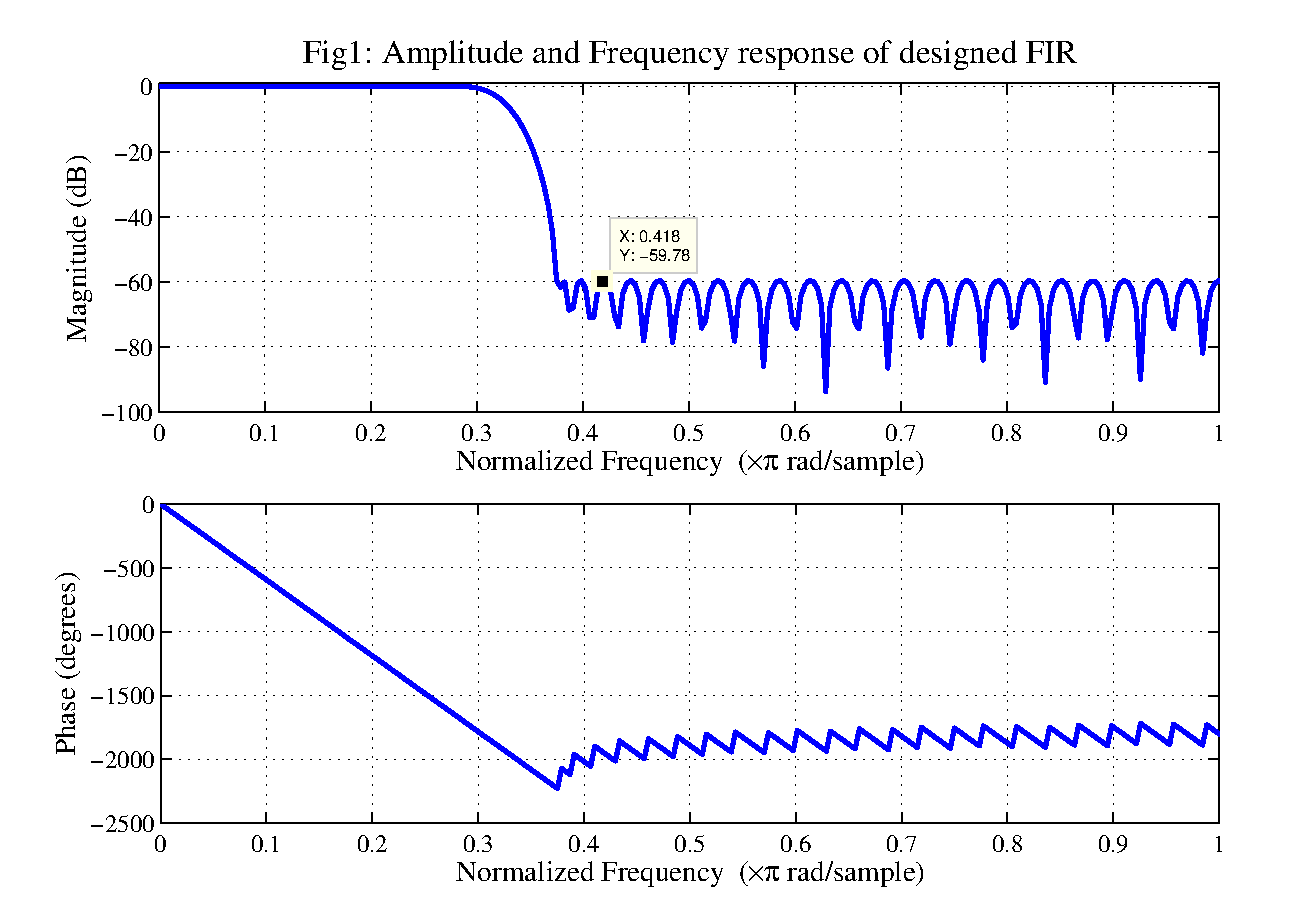
\includegraphics[width=1\textwidth]{fig1.eps}
\end{center}

在图1中可以看到设计好的滤波器是等波纹的,其阶数是$n=66$;滤波器在通带内不衰减,而在阻带的最小衰减达到了近$60dB$,过渡带较窄,符合我们的设计指标。此外,观察其相频函数可以发现设计好的FIR滤波器是线性相位的,这也符合我们的预期。程序代码可以在运行过程中给出设计滤波器系统函数的分子多项式系数,也即滤波器的抽头系数,分别为:

\begin{center}
\begin{tabular}{|c|c|c|c|c|c|c|}
\hline \multicolumn{7}{|c|}{$b_i$ = }\\
\hline 0.0013 & 0.0015 & 0.0007 & -0.0012 & -0.0026 & -0.0018 & 0.0010\\
\hline 0.0034 & 0.0024 & -0.0019 & -0.0057 & -0.0044 & 0.0019 & 0.0077\\
\hline 0.0064 & -0.0026 & -0.0113 & -0.0098 & 0.0028 & 0.0155 & 0.0143\\
\hline -0.0033 & -0.0222 & -0.0217 & 0.0035 & 0.0327 & 0.0344 & -0.0038\\
\hline -0.0549 & -0.0653 & 0.0038 & 0.1388 & 0.2732 & 0.3293 & 0.2732\\
\hline 0.1388 & 0.0038 & -0.0653 & -0.0549 & -0.0038 & 0.0344 & 0.0327\\
\hline 0.0035 & -0.0217 & -0.0222 & -0.0033 & 0.0143 & 0.0155 & 0.0028\\
\hline -0.0098 & -0.0113 & -0.0026 & 0.0064 & 0.0077 & 0.0019 & -0.0044\\
\hline -0.0057 & -0.0019 & 0.0024 & 0.0034 & 0.0010 & -0.0018 & -0.0026\\
\hline -0.0012 & 0.0007 & 0.0015 & 0.0013\\
\hline
\end{tabular}
\end{center}

在图2中,笔者画出了设计的FIR滤波器的零极点图。在图中可以清晰地看到其零点的分布,零点的出现也是共轭的。而FIR系统唯一的极点则是在$z=0$处出现,符合FIR系统收敛域的性质。由于这样的特性,FIR系统函数也是稳定的。
\begin{center}
    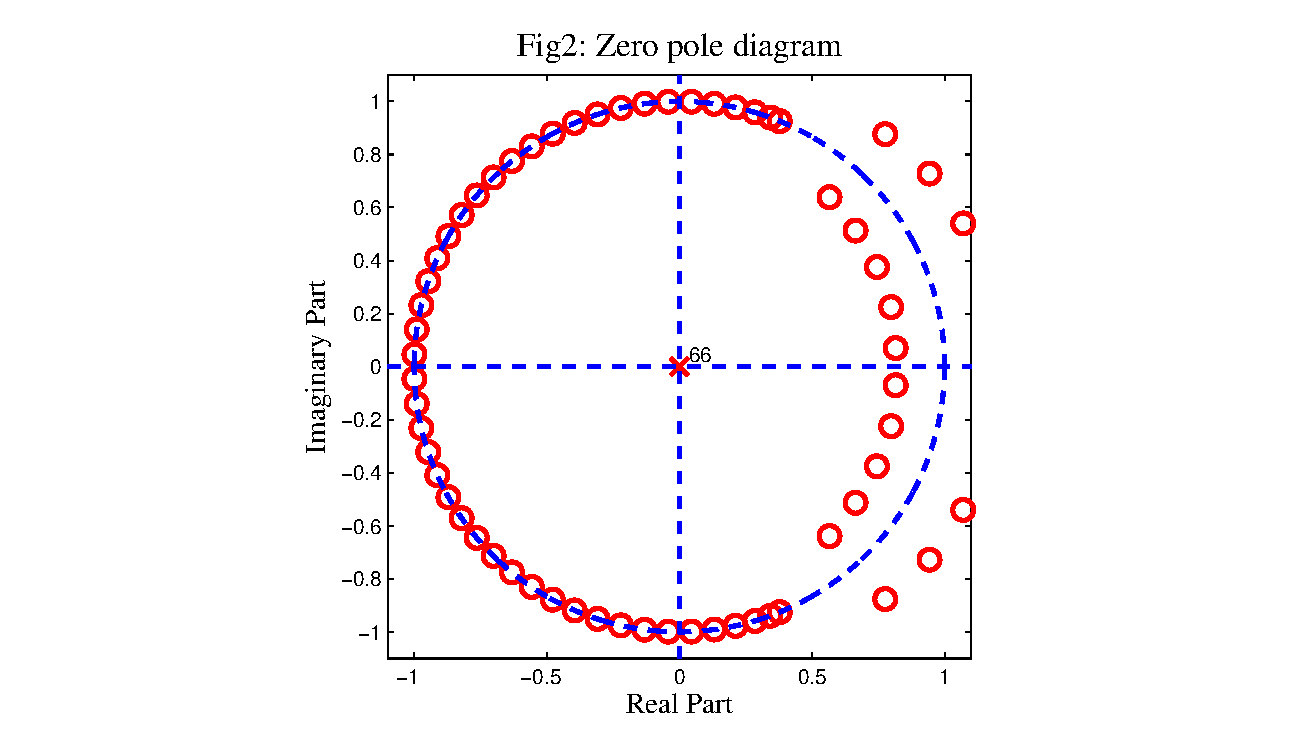
\includegraphics[width=1\textwidth]{fig2.eps}
\end{center}

在图3中,笔者画出了设计的FIR滤波器的群延迟。群延迟的定义为
\begin{equation}
\tau (\omega) = - \frac{d \varphi (\omega)}{d \omega}.
\end{equation}

在图中可以看出,对于此FIR滤波器而言,其群延迟对于所有的$\omega$都是常数,且满足
\begin{equation}
\tau (\omega) = \frac{N-1}{2} = 33,
\end{equation}
这就说明所设计的滤波器是具有线性相位函数的。
\begin{center}
    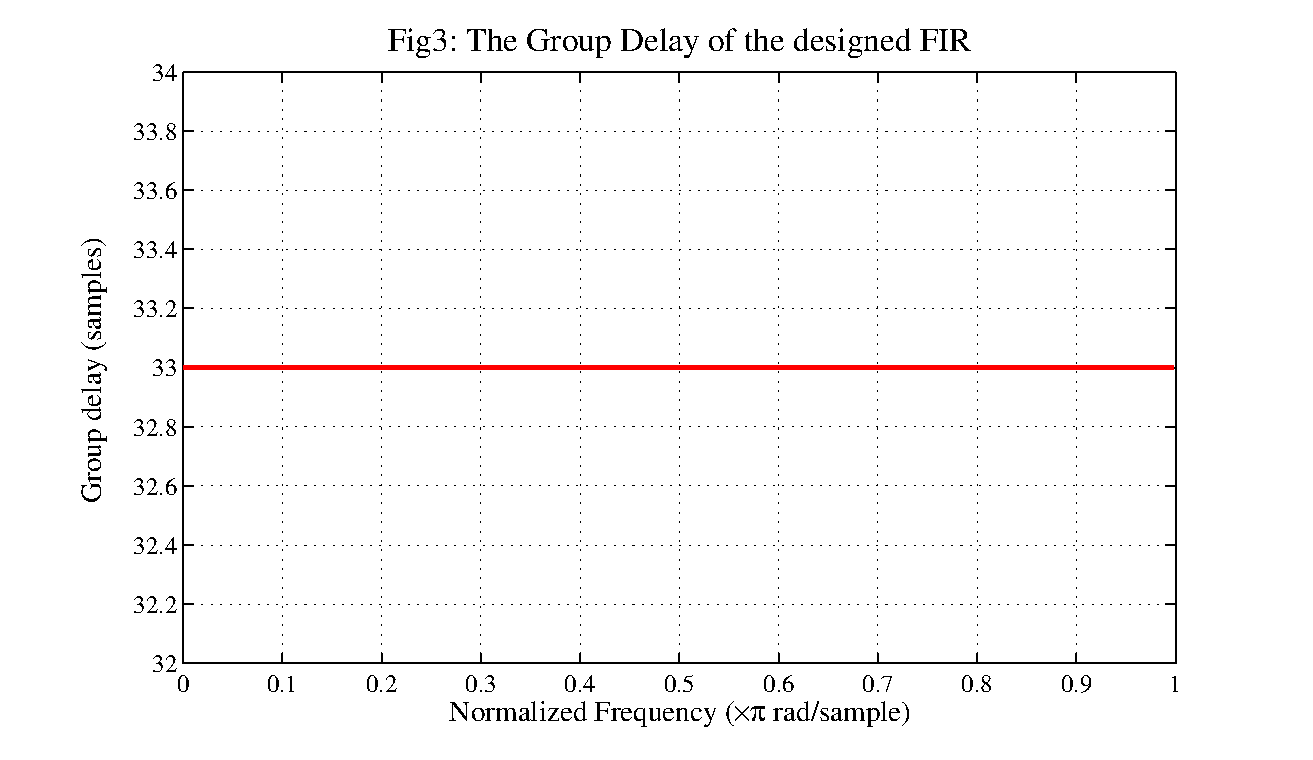
\includegraphics[width=1\textwidth]{fig3.eps}
\end{center}

\begin{center}
    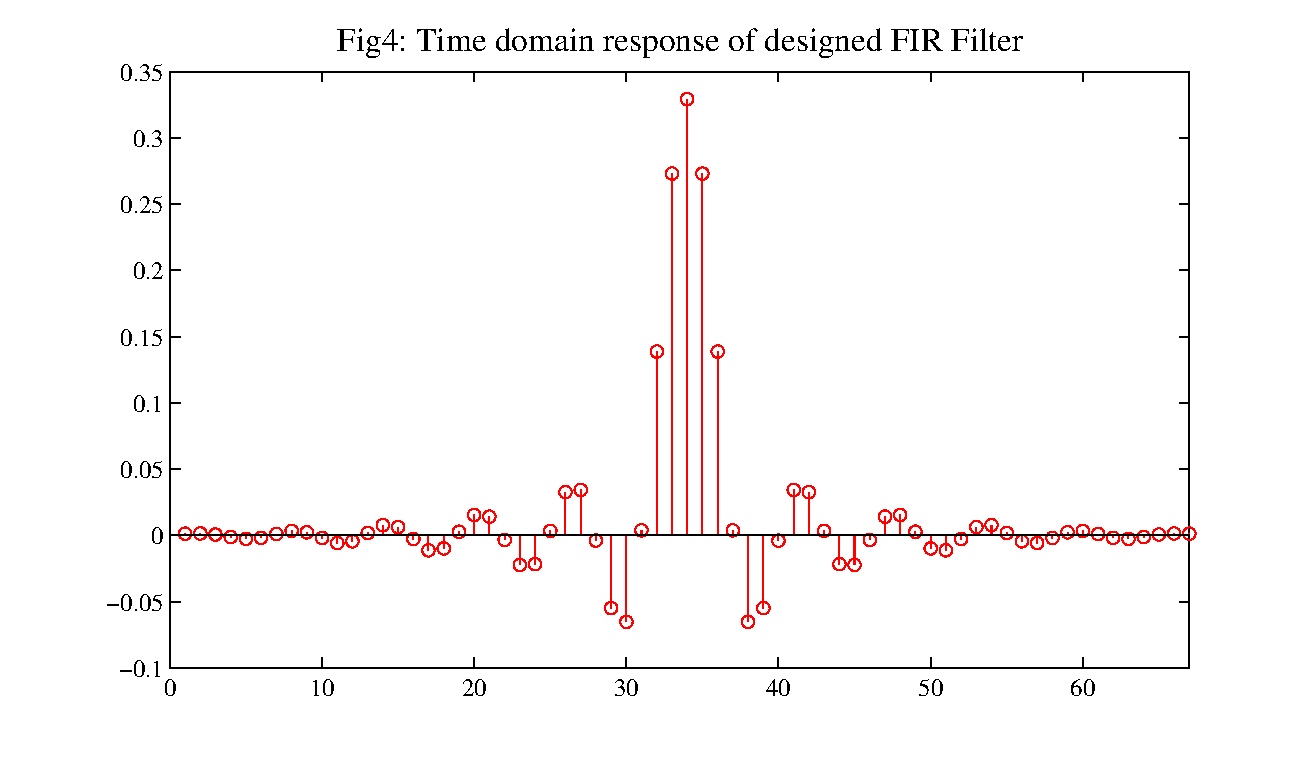
\includegraphics[width=1\textwidth]{fig4.eps}
\end{center}

在图4中,我们给出了此滤波器的时域响应。对于FIR滤波器而言,时域响应$h(n)$即是滤波器的抽头系数,即有
\begin{equation}
H(z) = \sum_{n=0}^{N-1} h(n) z^{-n}.
\end{equation}
从图中也可以看出其响应是有限长的,满足$N=67$。而仔细观察此冲激响应序列,不难发现其关于$\tau = \frac{N-1}{2}$呈偶对称,即抽头系数满足关系式
\begin{equation}
h(n) = h(N-1-n), \qquad \forall n \in [0, N-1].
\end{equation}

至此,完成了收、发端的FIR滤波器的设计。

\subsection{OFDM系统仿真实现}
完成了滤波器设计后,按照在第1.2.2节中所示的系统流程进行仿真~(具体代码见文件$OFDM.m$),并与BPSK调制的理论误码率进行比较,得到结果如图5 所示。其中BPSK 的理论误码率计算公式是
\begin{equation}
P_{bpsk} = \frac{1}{2} erfc(\sqrt{\frac{E_b}{N_0}})= Q(\sqrt{\frac{2E_b}{N_0}}).
\end{equation}

\begin{center}
    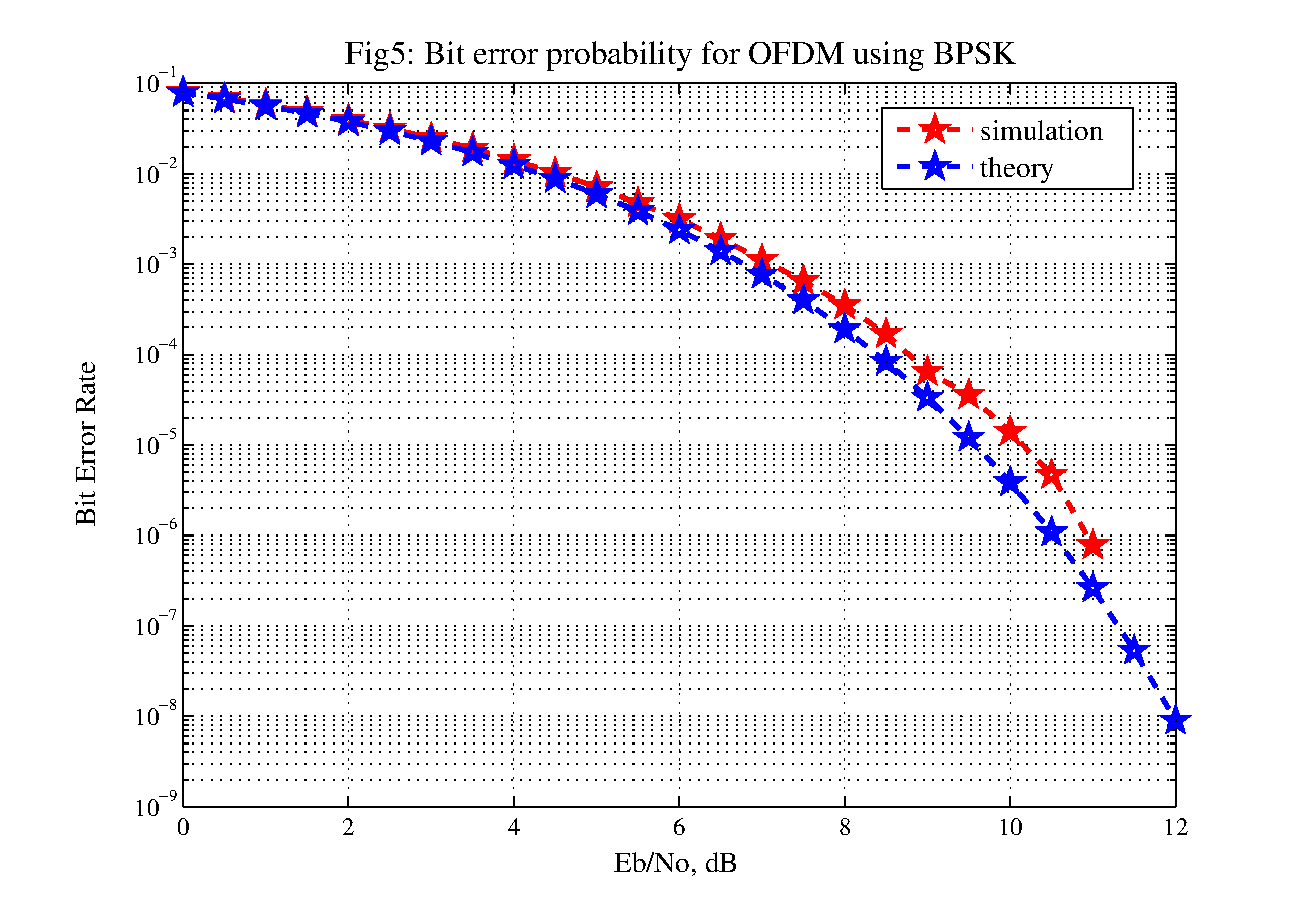
\includegraphics[width=1\textwidth]{fig5.eps}
\end{center}

从图中可以直观看到,随着$EbN0$的上升,OFDM系统的误码率逐渐下降,并且与理论误码率相近,在低信噪比的时候吻合良好,在高信噪比的时候存在一定的误码率上升,但无量级差别;考虑到输入的源信号数目足够大,说明此次仿真成功。至此,成功完成了OFDM的系统实现和仿真。

\vspace{0.2cm}
\section{实验结果分析}
在本节中,我们对本次实验的结果进行分析和更进一步的讨论。

\subsection{FIR滤波器设计}
FIR滤波器设计有多种方法,可以通过窗函数设计法~\supercite{course2},频率抽样设计法~\supercite{course3},最优化设计法~\supercite{course5}等等来得到。在$Matlab$中我们可以通过$fdatool$或是其字节提供的设计函数来得到相应的滤波器。

对于本次仿真给出的指标,我们采用频域最大绝对误差最小化准则,是有限单位脉冲响应滤波器的一种计算机辅助优化设计。窗口法设计和频率采样设计都存在某些缺陷。首先,在设计中不能将边缘频率$\omega_p$和$\omega_s$精确地给定。其次,不能够同时标定波纹因子$\delta_1$和$\delta_2$。最后,近似误差(即理想响应和实际响应之间的差)在频率区间上不是均匀分布的。而最优等纹波设计法能解决上面三个问题。

从设计结果中不难看出,阻带最小衰减达到了近60dB,而通带内则几乎是平滑不减的,过渡带的衰减也很快。对于FIR滤波器,要达到高设计要求,对应的阶数也会比同样参数的IIR滤波器要高~(本例中$N=67$)。而另一方面,在图1,图2和图3中可以看出FIR具有的明显优势是线性相位特点,对输入信号不会产生相位的畸变,而这一点在OFDM系统中则是至关重要的。另外,在图4中我们话除了此滤波器的时域响应,对比理想低通滤波的抽头系数:
\vspace{0.2cm}
\begin{equation}
h_d(n) = \frac{\omega_c}{\pi} \frac{\sin [ (n- \tau ) \omega_c ]}{(n- \tau ) \omega_c }, \qquad n \in (- \infty , \infty),
\end{equation}
其图像也是非常接近$sinc$函数的加有限窗形式。

\subsection{OFDM系统仿真实现}
OFDM给我最深的印象就是巧妙利用了$Nyquist$采样定律在多载波正交上的应用,使得载波之间无互相干扰。而这样做带来的弊端是需要对每一个OFDM符号进行过采样~(发射端进行上采样),使得其在通过数模转换~(DA)模块的时候不会发生畸变。

在本次试验中,利用BPSK调制,并经过高斯白噪声信道,最终的仿真结果比较满意,几乎与BPSK理论误码率一致。当$EbN0 = 0dB$时,误码率保持在0.1以下;随着信噪比的上升,误码率呈指数形式下降,在$EbN0 = 11dB$时,误码率已经下降至低于$10^{-6}$(由于精度问题,在$EbN0 > 11dB$时对数坐标轴无法表示,故最后两个点没有画出)。

对于仿真结果中与理论误码率存在一定差距的现象,主要原因我认为是FIR滤波器的设计采用的是所需要的最小阶数,而实际滤波器终归无法达到理想低通滤波器功能。此外,循环前缀CP的长度会影响到码间串扰和子载波见干扰,也对结果有一定影响~(本次试验中我取的$L=16$)。


\section{思考题}

\subsection{发端滤波器和收端滤波器的作用分别是什么}
由于OFDM系统需要对每一个OFDM符号进行上采样防止DA过程的失真,而过采样过程~(包括上采样和下采样)本身会对源信号频谱造成改变,故需要加上对应的滤波器。由于FIR滤波器具有多相结构这一特殊结构性质,故在防混叠滤波中有广泛的应用。

\subsubsection{发端滤波器}
对发射端而言,滤波前信号需要经过上采样,即8倍插值,在数字域中分析如下~\supercite{course6}:
\begin{equation}
\begin{split}
X_e(z) & = \sum_{n}x_e(n) z^{-n} = \sum_{n = 8k}x_e(\frac{n}{8})z^{-n} \\
& = \sum_{n}x(n)z^{-8n} = X(z^{8}), \\
X_e(e^{j\omega^{'}}) & = X(e^{j8\omega}), \qquad \omega^{'} = \frac{\omega}{8}.
\end{split}
\end{equation}
即插值后增加了新的频率分量,产生失真。为了防止这种失真出现,我们在上采样后插入平滑滤波器,又名插值中的平滑滤波~\supercite{course7},以滤去在基频中重复的镜像频率分量。其中此平滑滤波器的系统函数形式应为
\begin{equation}
H_I(e^{j\omega^{'}}) =
\left\{
\begin{aligned}
& 8, \qquad \big|\omega^{'}\big| < \frac{\pi}{8}, \\
& 0, \qquad else.
\end{aligned}
\right.
\end{equation}

由此,多速率信号抽样的上采样失真便可解决。

\subsubsection{收端滤波器}
对接收端而言,滤波前信号需要经过下采样,即8倍抽取,在数字域中分析如下~\supercite{course6}:
\begin{equation}
\begin{split}
X_d(z) & = \frac{1}{D} \sum_{n} \sum_{k=0}^{D-1} x(n) W_{D}^{-nk}z^{-\frac{n}{D}} \\
& = \frac{1}{D} \sum_{k=0}^{D-1} X(W_{D}^{k} z^{\frac{1}{D}}), \\
X_d(e^{j\omega^{'}}) & = \frac{1}{D} \sum_{k=0}^{D-1} X(e^{j\frac{\omega^{'}}{D}}e^{-j\frac{2k\pi}{D}}) \\
& = \frac{1}{D} \sum_{k=0}^{D-1} X(e^{j(\omega - \frac{2k\pi}{D})}), \qquad \omega^{'} = D\omega, \ D=8.
\end{split}
\end{equation}

抽样率越低,周期严拓后的频谱靠得越近,当$8\omega_h>\pi$时就会产生失真。为了防止这种失真出现,我们在下采样之前插入防混迭滤波器~\supercite{course7},以滤去在抽取后会发生混叠频率分量。其中此平滑滤波器的系统函数形式应为
\begin{equation}
H_d(e^{j\omega^{'}}) =
\left\{
\begin{aligned}
& 1, \qquad \big|\omega\big| < \frac{\pi}{8}, \\
& 0, \qquad else.
\end{aligned}
\right.
\end{equation}

由此,多速率信号抽样的下采样失真便可解决。综上所述,此两项即为收、发端低通滤波器的作用。

\subsection{系统带宽3M,128点IFFT,CP长度32,试分析当采用QPSK调制时,低通滤波器的参数是否需要改变,为什么?}
首先给出我的答案:不需要改变。对此题目我觉得有两种理解方式:1. 当采用QPSK调制时,OFDM子载波数目变为64,即一个OFDM符号含有64个QPSK调制符号~(因QPSK一个符号包含两比特信息,调制后符号数目减半);2. OFDM子载波数目保持不变,仍为128。

首先回顾思考题1中低通FIR滤波器的作用,是防止多速率抽样导致的信号频谱失真:对于上采样,需要保证$D\omega_h<\pi$,而下采样保持$L=D$即可。由于QPSK的本质是多进制编码调制,其频带利用效率相比于BPSK是升高的,即对于同样的比特流源信号~(传输码率$R_b$相同)有
\begin{equation}
B_{QPSK} = \frac{1}{\log 4} B_{BPSK} = \frac{1}{2} B_{BPSK}.
\end{equation}

故对于相同的上/下抽样速率,QPSK带宽要小一倍;当BPSK不发生混叠时,QPSK便不会发生混叠。即低通滤波器不需要改变。

为了验证此结论的正确性,我对QPSK在OFDM系统中的误码率进行了仿真,参数与BPSK时相同,且用的是同一低通滤波器。其中QPSK源信号生成代码如下:
% ===================================插入Matlab代码格式,参考matlab-prettifier文档
\begin{lstlisting}[style=Matlab-editor,
                   basicstyle=\mlttfamily,
                   caption={QPSK Modulation}, label=code3]
s_bit = round(rand(1,nBit_Sym*nSym));               % 随机0, 1比特序列
I_bit = 2*(s_bit(1:2:end) - 0.5);
Q_bit = 2*(s_bit(2:2:end) - 0.5);
s_bit_qpsk = I_bit + 1j*Q_bit;                      % QPSK调制:1+j, 1-j, -1+j, -1-j
s_bit_qpsk = reshape(s_bit_qpsk,nBit_Sym,nSym/2).';
\end{lstlisting}

\begin{center}
    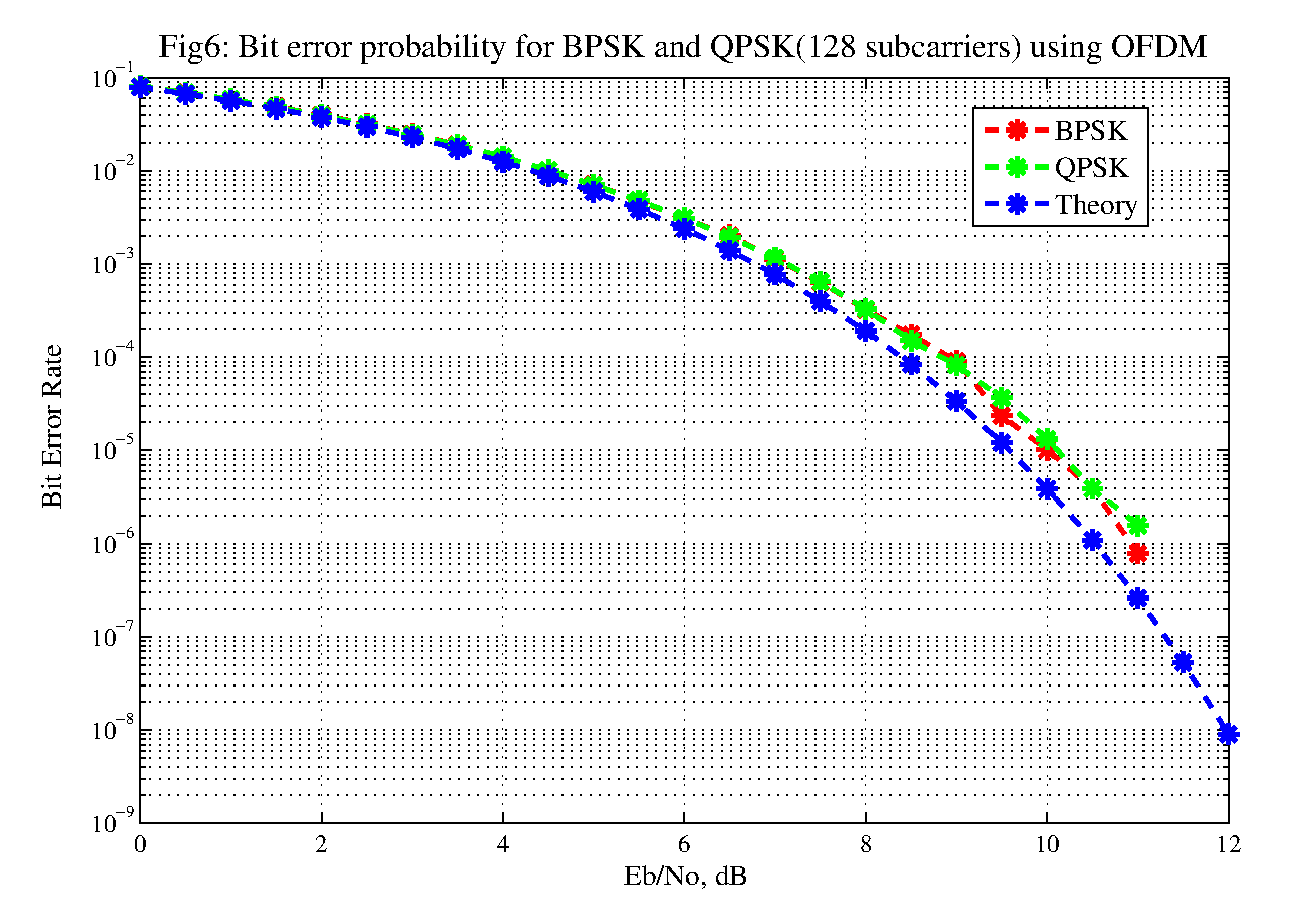
\includegraphics[width=1\textwidth]{fig6.eps}
\end{center}
\begin{center}
    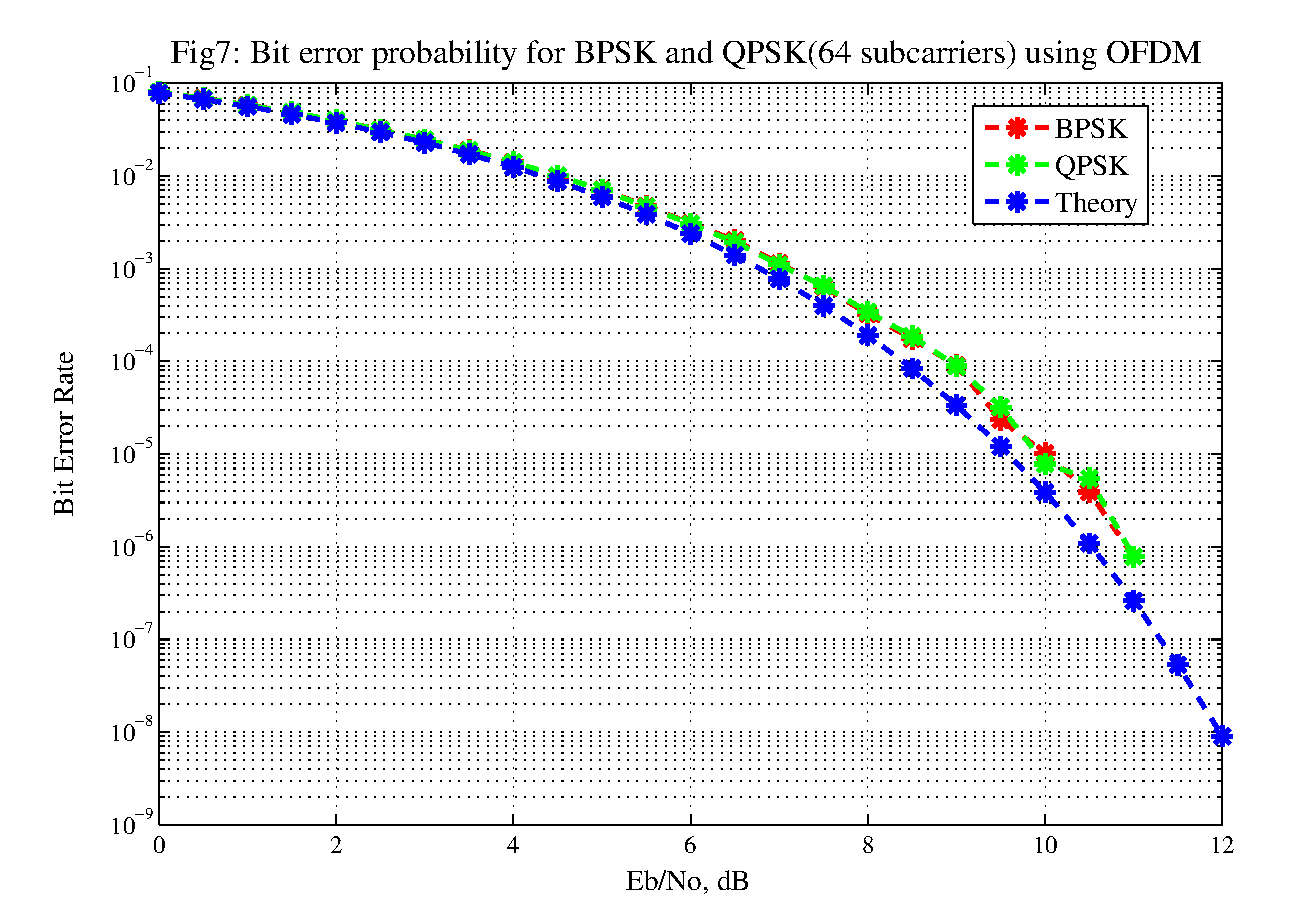
\includegraphics[width=1\textwidth]{fig7.eps}
\end{center}

仿真分别基于子载波数目为64和128,得到的结果分别如图6和图7所示。由图中可以看出BPSK和QPSK的误码率几乎一致,并且对于两个子载波数目都有此现象。同样的,由于两种调制方式的理论误码率是一致的,故在两个图中都可以看到BPSK和QPSK的误码率和理论误码率接近。至此,便验证了此结论的正确性。

这部分的代码在$OFDM\_QPSK\_BPSK.m$中实现。

\section{总结}

本次报告对关于$DFT$、$FFT$、OFDM系统和FIR滤波器等内容做了介绍,完整完成了FIR滤波器设计以及OFDM系统仿真过程,并给出了设计图和仿真结果图,最后对实验结果作出了详细的结果分析,用理论以及相应仿真回答了思考题。经过本次实验,本人对FIR滤波器设计有了更深的理解,对OFDM系统有了初步的了解与认识,并对较晦涩难懂的内容梳理得更加清楚。本次实验也让我学会了在通信系统的搭建仿真上如何一步一步处理,遇到BUG时该怎样改进代码,并分析失败原因,最终实现仿真预期目标。


\section{附录}
$Matlab$代码包括主文件$OFDM.m$以及fdatool导出的滤波器文件$my\_filter.m$~(在主文件中也用语句设计了滤波器),以及验证思考题实现的QPSK误码率仿真程序$OFDM\_QPSK\_BPSK.m$,其使用是添至搜索路径运行即可,其中代码具有详细的注释。

本文的图片均为$.eps$格式,可以进行缩放而不失真的矢量图,在观察某些细节(例如滤波器的响应等)时观察得更清楚。由于$Matlab$含有中文的图片在导出$.eps$ 文件时会出现乱码情况,故所有图片的标题等均为英文所写。

最后,由于报告中需要加入许多数学表达式,本文档使用了$LaTeX$来编写报告,以获得更优的排版效果。
\iffalse
\footnote{由于另一篇文章《学习心得与体会》我写的较为全面,涵盖了这部分的内容,所以两篇文章会有部分内容是一样的,但均为自己构思、写出的,可视作对前部分内容的加深、拓展。}。
\fi


% =====================================================Reference
\small
\begin{thebibliography}{99}
\setlength{\parskip}{0pt}  %段落之间的竖直距离

\bibitem{wiki}
https://zh.wikipedia.org/wiki.

\bibitem{textbook}
程佩青. 数字信号处理教程~(第三版), 清华大学出版社, 2012.6.

\bibitem{wikifft}
Brenner, N.; Rader, C. A New Principle for Fast Fourier Transformation. \emph{IEEE Acoustics, Speech \& Signal Processing}. 1976, 24(3): 264–266.

\bibitem{course1}
程宇新. 第4章, 滤波器概要, 数字滤波器结构2, FIR结构. 2017, 4.

\bibitem{course2}
程宇新. 第6章, FIR滤波器设计, 窗函数设计法. 2017, 5.

\bibitem{course3}
程宇新. 第6章, FIR滤波器设计, 频率抽样设计法. 2017, 5.

\bibitem{course4}
程宇新. 第6章, FIR滤波器设计, 线性相位FIR滤波器特点. 2017, 5.

\bibitem{course5}
程宇新. 第6章, FIR滤波器设计, 最优化设计法. 2017, 5.

\bibitem{course6}
程宇新. 第7章, 多速率信号处理, 信号的抽取和内插. 2017, 5.

\bibitem{course7}
程宇新. 第7章, 多速率信号处理, 抽取和内插滤波. 2017, 5.

\bibitem{ta}
TA. 数字信号处理第二次上机. 2017, 5.

\end{thebibliography}

\clearpage
\end{document}
